\chapter{Meccanica del Robot}
Il robot � costituito da tre diverse parti funzionali: una base dotata di ruote motrici,
 un braccio rotante ed un sistema di leve a forbice.

\section{La base}
La base del robot � stata costruita partendo da un modello presente sul sito
della \emph{Lego}\textregistered~
(\texttt{http://www.active-robots.com/products/mindstorms4schools/build\\ing-instructions/Build-RoboArm.pdf}
Figura \ref{Base}) e modificato come segue: il motore B, che nello schema originale si occupava di far ruotare il braccio, continua nella sua funzione mentre il motore A
trasferisce la sua funzione da far muovere in avanti il braccio a gestire la trazione del robot.\\

\begin{figure}
	\begin{center}
		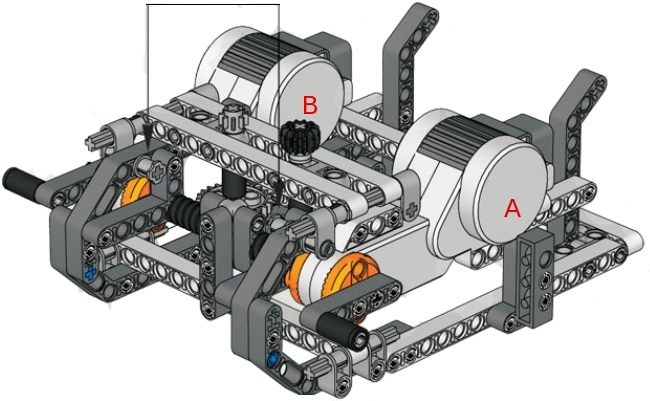
\includegraphics[scale=0.5]{img/base.png}
		\caption{Struttura iniziale della Base \label{Base}}
	\end{center}
\end{figure}

Per permettere al robot di avanzare, la base � stata montata su quattro ruote di
cui le due anteriori sono le ruote motrici. Queste ultime sono collegate tra di
loro con un asse motore comune, che riceve il movimento tramite un gioco di
ingranaggi conici trasformando la rotazione dall'asse verticale, prodotta dal
motore A pi� la vite archimedea, in un movimento sull'asse orizzontale
necessario per l'avanzamento del robot.\\

Questo sistema ha per� mostrato delle carenze di precisione dovute a torsioni,
flessioni e giochi meccanici.\\

Per ovviare a ci� si � proceduto in pi� modi: 
\begin{itemize} 
  \item Creando un nuovo sistema di aggancio dell'albero motore verticale, in
 		 modo da minimizzarne la flessione. Nello specifico, si � inserita una
  		 piastrina triangolare per 'agganciare' l'albero motore, il pi� vicino
  		 possibile al punto di contatto tra gli ingranaggi conici. Figura
  		 \ref{ALBERO}
  		 \begin{figure}
           \begin{center}
			 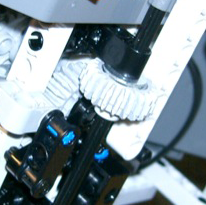
\includegraphics[scale=0.5]{img/trazione.png}
			 \caption{Aggancio albero motore e coppia di ingranaggi \label{ALBERO}}
		   \end{center}		
		 \end{figure}
 
  \item Inserendo sotto la base un asse rigido che arrivi da ruota a ruota, in
  		 modo da ridurre la flessione dell'albero motore, dovuta al peso del robot
  		 stesso.  Figura \ref{SOSPENSIONI} 
 
		\begin{figure}
         \begin{center}
			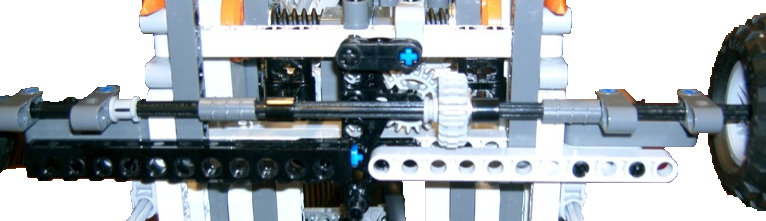
\includegraphics[scale=0.5]{img/sospensioni.png}
			\caption{Sospensioni anteriori\label{SOSPENSIONI}}
		  \end{center}
		\end{figure} 

  \item Inserendo delle parti non originali della 
  		\emph{Lego}\textregistered~per cercare di ridurre i giochi meccanici,
  		nello specifico si sono inserite delle rosette nella sede delle viti
  		achimedee e nei vari supporti degli assi. Figura \ref{ROSETTE} 
  		
  		\begin{figure}	
           \begin{center}	
			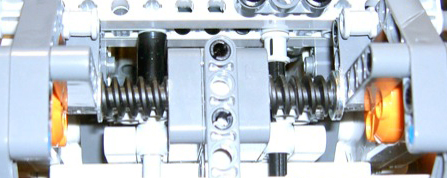
\includegraphics[scale=0.5]{img/rosette.jpg}
			\caption{Rosette per la riduzione dei giochi \label{ROSETTE}}
		  \end{center}			
		\end{figure}  	 


\end{itemize} 

Per i problemi relativi alle torsioni degli alberi non si � potuto fare nulla,
essendo questi problemi puramente dipendenti dalla natura fisica degli stessi e
non dal sistema di montaggio.
\section{Il Braccio}
Per la costruzione del braccio si � nuovamente presa ispirazione dalle
istruzioni della \emph{Lego}\textregistered, modificandolo in modo da renderlo
rigido e non pi� snodabile. Figura \ref{braccio1}.

  		\begin{figure}
          \begin{center}		
			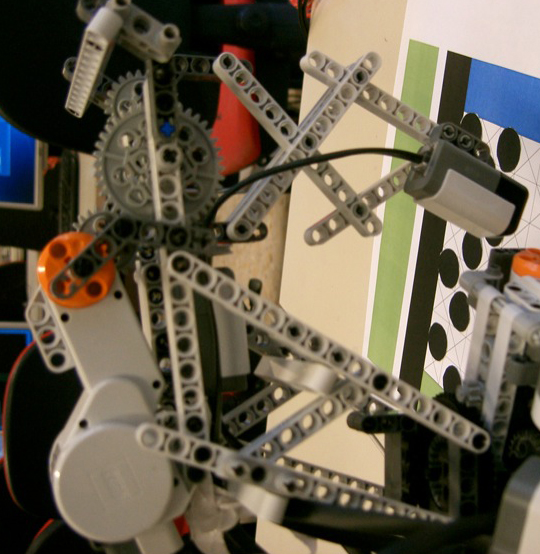
\includegraphics[scale=0.4]{img/foto_braccio.jpg}
			\caption{Immagine del Braccio completo \label{braccio1}}
		  \end{center}
		\end{figure} 

Per effettuare questa modifica si � elimitato il movimento centrale e fissati i
montanti del braccio tramite due 'traverse'. Figura \ref{braccio0}

  		\begin{figure}
          \begin{center}		
			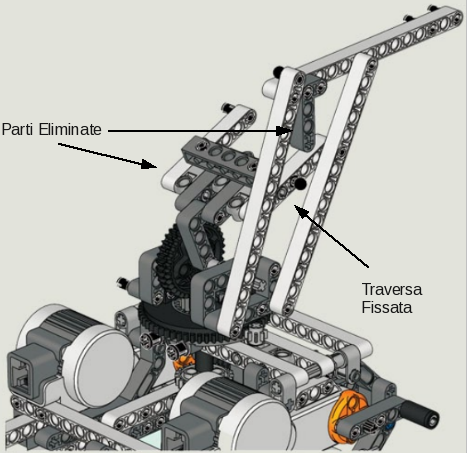
\includegraphics[scale=0.4]{img/braccio.png}
			\caption{Struttura del Braccio \label{braccio0}}
		  \end{center}
		\end{figure} 

Inoltre per dare maggior solidit� all'intera struttura si sono aggiunte delle
barre (\emph{Technic Beam}) che 'leghino' i due montanti insieme. Nello
specifico ne sono state montate tre: una sulla punta del braccio, una sul
montante anteriore ed una sul montante posteriore.

\section{Sistema di leve a forbice}

Per la costruzione della parte terminale del braccio si sono dovuti risolvere
due problemi: il primo ha riguardato il modo di generare un moto verticale, che abbassi la
punta del braccio da un moto rotatorio. Il secondo, e strettamente correlato al
primo, � stato quello di dare la giusta precisione in modo che il sensore sia
sempre alla stessa altezza dalla scacchiera. \\

Il primo problema si � deciso di risolverlo tramite un sitema di
leveraggi imperniati a forbice (in seguito per semplicit� denominato
\emph{pantografo}). Il pantografo prende il movimento da una coppia di
ingranaggi gemelli, ognuno montato rispettivamente nel punto di ancoraggio
delle braccia del pantografo. Figura \ref{leve}

  		\begin{figure}
          \begin{center}		
			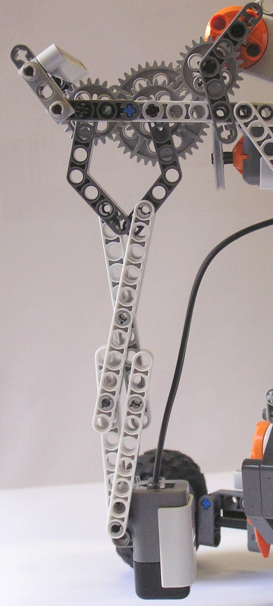
\includegraphics[scale=0.6]{img/leve.png}
			\caption{Sistema di leve a forbice \label{leve}}
		  \end{center}
		\end{figure} 

Per risolvere il problema della precisione nella discesa, problema in parte
risolto dall'adozione del pantografo, si � inserito un treno di ingranaggi
(Figura \ref{ingranaggi}) che riducono i giri del motore di 10
volte, in modo da ottenere un numero di giri sufficientemente elevato da
permettere una stima empirica del comando da impartire al motore.\\
  		\begin{figure}
          \begin{center}		
			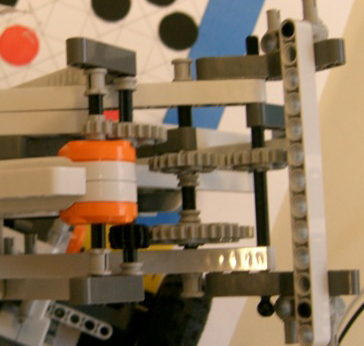
\includegraphics[scale=0.6]{img/ingranaggi.png}
			\caption{Treno di ingranaggi \label{ingranaggi}}
		  \end{center}
		\end{figure} 
Il pantografo � inoltre dotato di due sensori: il primo, situato sotto il treno
di ingranaggi, quindi solidale con il braccio, � il sensore di pressione
\emph{Electric Touch Sensor NXT} che viene premuto dalla prima leva quando il
pantografo � in alto. 
Il secondo � il sensore di colore \emph{NXT Color Sensor} che, posizionato alla
terminazione inferiore del pantografo, permette il riconoscimento dei colori.

